\documentclass[tikz,border=2pt]{standalone}
\usepackage{amsmath}
\usetikzlibrary{arrows.meta,positioning,calc}
\begin{document}
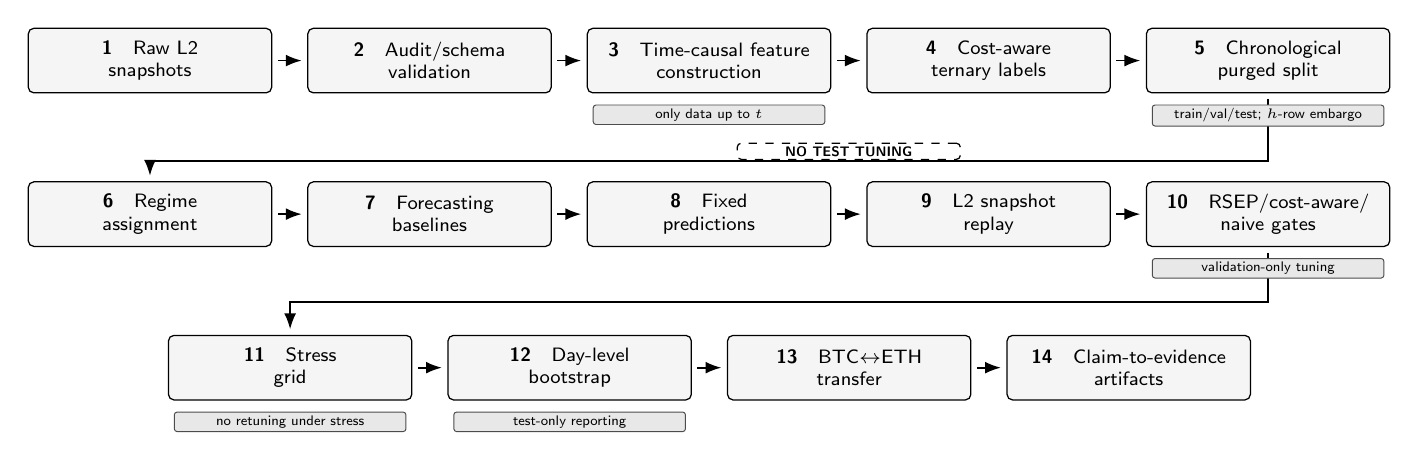
\begin{tikzpicture}[
  >=Latex,
  x=1cm,y=1cm,
  stage/.style={draw=black, rounded corners=2pt, line width=0.45pt, fill=gray!8,
    align=center, text width=2.95cm, minimum height=0.82cm, inner sep=2pt,
    font=\sffamily\scriptsize},
  note/.style={draw=black!70, rounded corners=1pt, line width=0.35pt, fill=gray!18,
    align=center, text width=2.85cm, inner sep=1.3pt, font=\sffamily\tiny},
  guard/.style={draw=black, dashed, rounded corners=1.5pt, line width=0.45pt,
    fill=white, align=center, text width=2.75cm, inner sep=1.2pt,
    font=\sffamily\tiny\bfseries},
  arrow/.style={->, line width=0.6pt, shorten >=2pt, shorten <=2pt}
]

% Row 1: data, targets, and split
\node[stage] (s1) at (0,0) {\textbf{1}\quad Raw L2\\snapshots};
\node[stage] (s2) at (3.55,0) {\textbf{2}\quad Audit/schema\\validation};
\node[stage] (s3) at (7.10,0) {\textbf{3}\quad Time-causal feature\\construction};
\node[stage] (s4) at (10.65,0) {\textbf{4}\quad Cost-aware\\ternary labels};
\node[stage] (s5) at (14.20,0) {\textbf{5}\quad Chronological\\purged split};

% Row 2: diagnostics, predictors, and replay policy
\node[stage] (s6) at (0,-1.95) {\textbf{6}\quad Regime\\assignment};
\node[stage] (s7) at (3.55,-1.95) {\textbf{7}\quad Forecasting\\baselines};
\node[stage] (s8) at (7.10,-1.95) {\textbf{8}\quad Fixed\\predictions};
\node[stage] (s9) at (10.65,-1.95) {\textbf{9}\quad L2 snapshot\\replay};
\node[stage] (s10) at (14.20,-1.95) {\textbf{10}\quad RSEP/cost-aware/\\naive gates};

% Row 3: robustness, uncertainty, transfer, and evidence
\node[stage] (s11) at (1.78,-3.90) {\textbf{11}\quad Stress\\grid};
\node[stage] (s12) at (5.33,-3.90) {\textbf{12}\quad Day-level\\bootstrap};
\node[stage] (s13) at (8.88,-3.90) {\textbf{13}\quad BTC$\leftrightarrow$ETH\\transfer};
\node[stage] (s14) at (12.43,-3.90) {\textbf{14}\quad Claim-to-evidence\\artifacts};

% In-row arrows
\draw[arrow] (s1) -- (s2);
\draw[arrow] (s2) -- (s3);
\draw[arrow] (s3) -- (s4);
\draw[arrow] (s4) -- (s5);
\draw[arrow] (s6) -- (s7);
\draw[arrow] (s7) -- (s8);
\draw[arrow] (s8) -- (s9);
\draw[arrow] (s9) -- (s10);
\draw[arrow] (s11) -- (s12);
\draw[arrow] (s12) -- (s13);
\draw[arrow] (s13) -- (s14);

% Row transition arrows preserve the sequential path while keeping the figure compact.
\draw[arrow] (s5.south) -- ++(0,-0.86) -| (s6.north);
\draw[arrow] (s10.south) -- ++(0,-0.70) -| (s11.north);

% Leakage and tuning guards
\node[note, below=0.14cm of s3] {only data up to $t$};
\node[note, below=0.14cm of s5] {train/val/test; $h$-row embargo};
\node[guard] at ($(s8.north)!0.5!(s9.north)+(0,0.38)$) {NO TEST TUNING};
\node[note, below=0.14cm of s10] {validation-only tuning};
\node[note, below=0.14cm of s11] {no retuning under stress};
\node[note, below=0.14cm of s12] {test-only reporting};

\end{tikzpicture}
\end{document}
